% Options for packages loaded elsewhere
\PassOptionsToPackage{unicode}{hyperref}
\PassOptionsToPackage{hyphens}{url}
\PassOptionsToPackage{dvipsnames,svgnames,x11names}{xcolor}
%
\documentclass[
  authoryear,
  preprint,
  3p]{elsarticle}

\usepackage{amsmath,amssymb}
\usepackage{iftex}
\ifPDFTeX
  \usepackage[T1]{fontenc}
  \usepackage[utf8]{inputenc}
  \usepackage{textcomp} % provide euro and other symbols
\else % if luatex or xetex
  \usepackage{unicode-math}
  \defaultfontfeatures{Scale=MatchLowercase}
  \defaultfontfeatures[\rmfamily]{Ligatures=TeX,Scale=1}
\fi
\usepackage{lmodern}
\ifPDFTeX\else  
    % xetex/luatex font selection
\fi
% Use upquote if available, for straight quotes in verbatim environments
\IfFileExists{upquote.sty}{\usepackage{upquote}}{}
\IfFileExists{microtype.sty}{% use microtype if available
  \usepackage[]{microtype}
  \UseMicrotypeSet[protrusion]{basicmath} % disable protrusion for tt fonts
}{}
\makeatletter
\@ifundefined{KOMAClassName}{% if non-KOMA class
  \IfFileExists{parskip.sty}{%
    \usepackage{parskip}
  }{% else
    \setlength{\parindent}{0pt}
    \setlength{\parskip}{6pt plus 2pt minus 1pt}}
}{% if KOMA class
  \KOMAoptions{parskip=half}}
\makeatother
\usepackage{xcolor}
\setlength{\emergencystretch}{3em} % prevent overfull lines
\setcounter{secnumdepth}{5}
% Make \paragraph and \subparagraph free-standing
\ifx\paragraph\undefined\else
  \let\oldparagraph\paragraph
  \renewcommand{\paragraph}[1]{\oldparagraph{#1}\mbox{}}
\fi
\ifx\subparagraph\undefined\else
  \let\oldsubparagraph\subparagraph
  \renewcommand{\subparagraph}[1]{\oldsubparagraph{#1}\mbox{}}
\fi


\providecommand{\tightlist}{%
  \setlength{\itemsep}{0pt}\setlength{\parskip}{0pt}}\usepackage{longtable,booktabs,array}
\usepackage{calc} % for calculating minipage widths
% Correct order of tables after \paragraph or \subparagraph
\usepackage{etoolbox}
\makeatletter
\patchcmd\longtable{\par}{\if@noskipsec\mbox{}\fi\par}{}{}
\makeatother
% Allow footnotes in longtable head/foot
\IfFileExists{footnotehyper.sty}{\usepackage{footnotehyper}}{\usepackage{footnote}}
\makesavenoteenv{longtable}
\usepackage{graphicx}
\makeatletter
\def\maxwidth{\ifdim\Gin@nat@width>\linewidth\linewidth\else\Gin@nat@width\fi}
\def\maxheight{\ifdim\Gin@nat@height>\textheight\textheight\else\Gin@nat@height\fi}
\makeatother
% Scale images if necessary, so that they will not overflow the page
% margins by default, and it is still possible to overwrite the defaults
% using explicit options in \includegraphics[width, height, ...]{}
\setkeys{Gin}{width=\maxwidth,height=\maxheight,keepaspectratio}
% Set default figure placement to htbp
\makeatletter
\def\fps@figure{htbp}
\makeatother

\makeatletter
\@ifpackageloaded{caption}{}{\usepackage{caption}}
\AtBeginDocument{%
\ifdefined\contentsname
  \renewcommand*\contentsname{Table of contents}
\else
  \newcommand\contentsname{Table of contents}
\fi
\ifdefined\listfigurename
  \renewcommand*\listfigurename{List of Figures}
\else
  \newcommand\listfigurename{List of Figures}
\fi
\ifdefined\listtablename
  \renewcommand*\listtablename{List of Tables}
\else
  \newcommand\listtablename{List of Tables}
\fi
\ifdefined\figurename
  \renewcommand*\figurename{Figure}
\else
  \newcommand\figurename{Figure}
\fi
\ifdefined\tablename
  \renewcommand*\tablename{Table}
\else
  \newcommand\tablename{Table}
\fi
}
\@ifpackageloaded{float}{}{\usepackage{float}}
\floatstyle{ruled}
\@ifundefined{c@chapter}{\newfloat{codelisting}{h}{lop}}{\newfloat{codelisting}{h}{lop}[chapter]}
\floatname{codelisting}{Listing}
\newcommand*\listoflistings{\listof{codelisting}{List of Listings}}
\makeatother
\makeatletter
\makeatother
\makeatletter
\@ifpackageloaded{caption}{}{\usepackage{caption}}
\@ifpackageloaded{subcaption}{}{\usepackage{subcaption}}
\makeatother
\journal{Palaeo3}
\ifLuaTeX
  \usepackage{selnolig}  % disable illegal ligatures
\fi
\usepackage[]{natbib}
\bibliographystyle{elsarticle-harv}
\usepackage{bookmark}

\IfFileExists{xurl.sty}{\usepackage{xurl}}{} % add URL line breaks if available
\urlstyle{same} % disable monospaced font for URLs
\hypersetup{
  pdftitle={Interspecies comparisons of Mg/Ca ratios in limpet shells},
  pdfauthor={Niklas Hausmann; Donna Surge; Francisco Zangrando; Angelica Tivoli; Ivan Briz-Godino},
  pdfkeywords={Sclerochronology, Limpets, Elemental Ratio, Mg/Ca},
  colorlinks=true,
  linkcolor={blue},
  filecolor={Maroon},
  citecolor={Blue},
  urlcolor={Blue},
  pdfcreator={LaTeX via pandoc}}

\setlength{\parindent}{6pt}
\begin{document}

\begin{frontmatter}
\title{Interspecies comparisons of Mg/Ca ratios in limpet shells}
\author[1]{Niklas Hausmann%
\corref{cor1}%
}
 \ead{niklas@palaeo.eu} 
\author[2]{Donna Surge%
%
}

\author[3]{Francisco Zangrando%
%
}

\author[3]{Angelica Tivoli%
%
}

\author[4]{Ivan Briz-Godino%
%
}


\affiliation[1]{organization={Leibniz Zentrum für
Archäologie},addressline={Ludwig-Lindenschmit-Forum
1},city={Mainz},country={Germany},countrysep={,},postcode={55116},postcodesep={}}
\affiliation[2]{organization={University of North
Carolina},addressline={104 South Road, 225 Geology
Building},city={Chapel Hill,
NC},country={US},countrysep={,},postcode={27599-3315},postcodesep={}}
\affiliation[3]{organization={CONICET (Consejo Nacional de
Investigaciones Científicas y Técnicas)},addressline={Avenida Maipú
305},city={Ushuaia},country={Argentina},countrysep={,},postcode={V9410BJA},postcodesep={}}
\affiliation[4]{organization={},country={Spain},countrysep={,},postcodesep={}}

\cortext[cor1]{Corresponding author}





        
\begin{abstract}
This study provides a short reassessment of the use of Magnesium to
Calcium (Mg/Ca) ratios in Atlantic limpet shells to determine past sea
surface temperatures. While \emph{Patella vulgata} along the Spanish
shoreline has since then repeatedly produced reliable correlations
between sea surface temperature and Mg/Ca ratios, this is not the case
for other patelloid species. \emph{Patella vulgata} and \emph{Nacella
deaureata} have been studied using Mg/Ca with mixed or contrary results.
In this study, we present elemental maps of various such species
together with stable oxygen isotope values for some of the specimens.
Our dataset also includes specimens that were previously unsuccessful in
providing significant correlations between δ\textsuperscript{18}O and
Mg/Ca ratios. By reassessing these previous specimens and including a
wider range of modern and archaeological samples from three patelloid
species (\emph{P. vulgata}, \emph{N. deaureata}, and \emph{N.
magellanica}) we further add to the growing set of evidence for the
reliable use of Mg/Ca ratios to detect palaeotemperature change and
serve as a means to determine ontogenetic age and season of capture as
well as to reveal locations of interest within the growth record
(i.e.~annual temperature minima and maxima) for the targeted analysis
using δ\textsuperscript{18}O or clumped oxygen isotope analysis.
\end{abstract}





\begin{keyword}
    Sclerochronology \sep Limpets \sep Elemental Ratio \sep 
    Mg/Ca
\end{keyword}
\end{frontmatter}
    
\section{Introduction}\label{Introduction}

Limpet shells are commonly found within archaeological sites and and
past shorelines due to their robust carbonate structure and the
long-term use of limpets as a marine food source. They have successfully
been studied in the past in the context of coastal subsistence
economies, site occupation on seasonal
\citep{Shackleton1973-ij, Parker2018-wf, Bosch2018-ud} or long-term
scale \citep{Ortiz2015-mr}, as well as palaeotemperature
\citep{Fenger2007-gf, Surge2012-ba, Wang2012-ee, Colonese2012-ct, Ferguson2011-zl}.
Determining past sea surface temperature (SST) change largely relies on
the measurement of δ\textsuperscript{18}O-values within the calcitic
parts of the shell, but attempts have been made to also use elemental
ratios, such as magnesium to calcium (Mg/Ca), to have an alternative
measure, that potentially provides a more accurate SST estimate than
δ\textsuperscript{18}O-values, which are also affected by changes in
salinity. In addition, the data acquisition of elemental ratios ---
either through laser-ablation-isotope-ratio-mass-spectrometry
(LA-ICP-MS) or laser induced breakdown spectroscopy (LIBS), can be much
faster and cost-effective, increasing the number of specimens that can
be studied overall \citep{Durham2017-fh, Hausmann2023-ih}.

Problematically, links between Mg/Ca ratios and SST changes in many
marine mollusc shells, including limpets, have shown to be unreliable
\citep{Surge2008-ri, Wanamaker2008-zl, Schone2010-yl, Freitas2012-tx, Graniero2015-zv, Poulain2015-dg, Vihtakari2017-wd}.
This is particularly the case where there is little available additional
information on metabolic processes, organic components of the shell
matrix, intra-increment and intra-shell variability, and growth rates,
which can independently and unpredictably affect Mg/Ca ratios and
confound their interpretation as temperature proxy. Confusingly,
multiple different temperature equations have been found for the same
species (see \citep{Freitas2012-tx, Vihtakari2017-wd} and references
therein). Coeval specimens sharing one locality can also show
differences in their relation to SST \citep{Hausmann2019-fi}. Where the
use of Mg/Ca as a palaeotemperature proxy was successful, anomalous
patterns in some specimens had still to be filtered out by hand,
reducing the overall robustness of the results of those successful
studies \citep{Ferguson2011-zl}.

While recent research particularly of \emph{Patella} sp. in the
Mediterranean and Southwest Europe have provided promising results
\citep{Hausmann2019-fi, Garcia-Escarzaga2015-jc, Garcia-Escarzaga2018-nf}.
There remains a lack of clarity for Atlantic limpet species,
particularly since it was last shown here, that they are not reliable
recorders of palaeotemperature \citep{Graniero2015-zv}.

In this study we will repeat and expand the analysis of Atlantic limpets
to determine the reliability of Mg/Ca ratios as palaeotemperature
proxies. To do this, we sampled a set of previously published and
unpublished limpet specimens dating to modern and archaeological
contexts using LIBS. LIBS allows us to carry out 2D imaging of entire
shell sections, which helps us to navigate the complex elemental
structure of the shell and better separate the external,
temperature-related changes from the internal and less understood
factors that influence the Mg/Ca ratio.

By relying and adding onto published datasets, we were able to
simultaneously avoid costs for new high-resolution
δ\textsuperscript{18}O-data, to use real-world examples, and to also
provide pilot-data for areas of existing research interest. Generally
establishing the usefulness and reliability of Mg/Ca as SST proxy in
limpets should help to provide a platform for future research and an
important stepping stone to better understand elemental ratios in other
marine mollusc shells.

\section{Materials and Methods}\label{Methods}

\subsection{Limpet specimens}\label{limpet-specimens}

\subsubsection{Modern specimens}\label{modern-specimens}

The analysed specimens, their origin and respective studies with
research background information can be found in \hyperref[Table_1]{Table
1}. Here we will briefly summarise their contextual information, which
can be accessed in more detail at the respective studies
\citep{Nicastro2020-ih, Surge2012-ba, Graniero2017-io}. While those
studies also included other specimens, their accessibility or state of
preservation did not all lend them to be re-analysed.

\phantomsection\label{Table_1}
\begin{longtable}[]{@{}
  >{\raggedright\arraybackslash}p{(\columnwidth - 10\tabcolsep) * \real{0.1667}}
  >{\raggedright\arraybackslash}p{(\columnwidth - 10\tabcolsep) * \real{0.1667}}
  >{\raggedright\arraybackslash}p{(\columnwidth - 10\tabcolsep) * \real{0.1667}}
  >{\raggedright\arraybackslash}p{(\columnwidth - 10\tabcolsep) * \real{0.1667}}
  >{\raggedright\arraybackslash}p{(\columnwidth - 10\tabcolsep) * \real{0.1667}}
  >{\raggedright\arraybackslash}p{(\columnwidth - 10\tabcolsep) * \real{0.1667}}@{}}
\caption{Overview of the modern and archaeological limpet specimens
analysed in this study.}\tabularnewline
\toprule\noalign{}
\begin{minipage}[b]{\linewidth}\raggedright
Context
\end{minipage} & \begin{minipage}[b]{\linewidth}\raggedright
Study
\end{minipage} & \begin{minipage}[b]{\linewidth}\raggedright
Species
\end{minipage} & \begin{minipage}[b]{\linewidth}\raggedright
Location
\end{minipage} & \begin{minipage}[b]{\linewidth}\raggedright
Sample ID
\end{minipage} & \begin{minipage}[b]{\linewidth}\raggedright
Previous analyses
\end{minipage} \\
\midrule\noalign{}
\endfirsthead
\toprule\noalign{}
\begin{minipage}[b]{\linewidth}\raggedright
Context
\end{minipage} & \begin{minipage}[b]{\linewidth}\raggedright
Study
\end{minipage} & \begin{minipage}[b]{\linewidth}\raggedright
Species
\end{minipage} & \begin{minipage}[b]{\linewidth}\raggedright
Location
\end{minipage} & \begin{minipage}[b]{\linewidth}\raggedright
Sample ID
\end{minipage} & \begin{minipage}[b]{\linewidth}\raggedright
Previous analyses
\end{minipage} \\
\midrule\noalign{}
\endhead
\bottomrule\noalign{}
\endlastfoot
Modern & \citep{Nicastro2020-ih} & \emph{N. deaureata} & Cambaceres Bay
- Tierra del Fuego (AR) & ND-1016-3 & Stable oxygen and carbon isotope
analysis \\
& & & & ND-1016-4 & \\
& & \emph{N. magellanica} & & NM-1016-1 & \\
& & & & NM-1016-3 & \\
& \citep{Graniero2017-io} & \emph{P. vulgata} & Rack Wick Bay - Westray
(UK) & ORK-LT5 & Stable oxygen and carbon isotope analysis; Mg, Li, Sr,
Ca,. \\
Archaeological & \citep{Surge2012-ba} & \emph{P. vulgata} & Rack Wick
Bay - Westray (UK) & QG1-7188-1 & Stable oxygen and carbon isotope
analysis \\
& & & & QG1-7189-2 & \\
& & & & QG2-1061-1 & \\
& & & & QG2-1064-1 & \\
& & & & QG2-7180-1 & \\
& & & & QG2-7180-2 & \\
& & & & QG1-7246-1 & \\
& This study & \emph{N. magellanica} & Heshkaia 35 in Moat Bay - Tierra
del Fuego (AR) & Heshkaia\_35-1 & \emph{none} \\
& & \emph{N. deaureata} & & Heshkaia\_35-2 & \\
& & \emph{N. deaureata} & & Heshkaia\_35-3 & \\
& & \emph{N. magellanica} & & Heshkaia\_35-4 & \\
& & \emph{N. magellanica} & & Heshkaia\_35-5 & \\
& & \emph{N. magellanica} & & Heshkaia\_35-6 & \\
& & \emph{N. magellanica} & & Heshkaia\_35-7 & \\
& & \emph{N. deaureata} & & Heshkaia\_35-8 & \\
& & \emph{N. magellanica} & & Heshkaia\_35-9 & \\
\end{longtable}

There are two main locations that we sourced specimens from: the Beagle
Channel in Tierra del Fuego (Argentina) and the island of West Ray in
Orkney (UK). Four specimens were collected from the Beagle Channel in
Cambaceres Bay in October 2016. The area receives around 570 mm
precipitation but the channel waters are predominantly influenced by
marine currents and in the period of October 2015 to October 2016 stayed
around 30.7 ± 0.7 psu \citep{Nicastro2020-ih}. SSTs range from 4.7ºC in
August to 10ºC in February.

On Westray one modern shell (ORK-LT5) was collected in Rack Wick Bay in
August 2009. Westray lies about 70 km north of the Scottish mainland and
experiences virtually no freshwater input with salinity values of 34.0
-- 34.5 psu \citep{Inall2009-ho}. The annual SST ranges from 6.3ºC in
March to 13.8ºC in August (Figure~\ref{fig-SSTs}).

\begin{figure}

\centering{

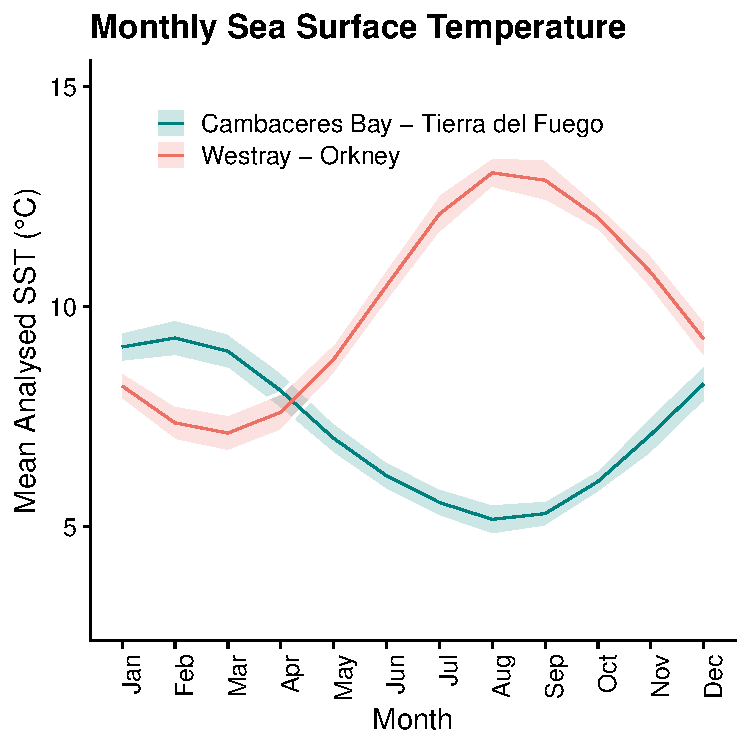
\includegraphics{Manuscript_files/figure-pdf/fig-SSTs-1.pdf}

}

\caption{\label{fig-SSTs}SST values averaged from years. SST values were
sourced from \citet{Good2020-nl}}

\end{figure}%

\subsubsection{Archaeological specimens}\label{archaeological-specimens}

In total, we studied 16 archaeological specimens. Of those, seven
\emph{P. vulgata} come from Quoygrew on Westray dating to 900 -- 1200
CE. These shells have previously been studied to characterise seasonal
temperature change during the Medieval Climate Anomaly and the Little
Ice Age \citep{Surge2012-ba}. Together they show a range of lifespans,
with some comparatively long for their size (QG1-7246-1, 12 years within
16 mm of growth) making them particularly susceptible to time-averaging.
That said, the majority are under 5 years old. These shells are an ideal
comparative dataset from an archaeological assemblage to compare to the
modern shell ORK\_LT5 \citep{Graniero2017-io}.

Nine additional shells of \emph{N. magellanica} (n=6) and \emph{N}.
\emph{deaureata} (n=3) have been selected for LIBS analysis only, to
provide a comparative dataset to the modern \emph{Nacella} sp. shells.
These have not been analysed for δ\textsuperscript{18}O-values, but
rather as a test to see whether patterns visible in the modern Mg/Ca
ratio distributions are also preserved and apparent in the
archaeological shells. They derive from the site of Heshkaia 35 situated
within Moat Bay, around 30 km east of where the modern specimens in our
study were collected \citep{Zangrando2014-qi, Zangrando2021-qg}. With
radiocarbon dates putting the shells into the Late Holocene (1300 --
1450 CE) they are of similar age --- if somewhat younger --- as the
assemblage from Quoygrew.

\subsection{Methods}\label{methods}

\subsubsection{Mg/Ca ratios}\label{mgca-ratios}

Mg/Ca elemental imaging was carried out using Laser Induced Breakdown
Spectroscopy at the Leibniz Zentrum für Archäologie (Mainz-Germany)
using previously published methods \citep{Hausmann2023-ih}. These
involve the ablation of the shell section using an infrared (1064 nm)
laser (1--2 mJ, 100 Hz) onto a surface area of 20--30 µm to generate a
plasma plume. This plume emits light, which is measured using a
synchronised spectrometer. The resulting light spectrum quantifies the
emission lines of magnesium (MgII; 279.553 nm) and calcium (CaII;
315.887 nm) to determine their intensity ratio. While these two peaks
alone do not represent the molar concentrations of both elements (as
opposed to calibration free LIBS; e.g.
\citep{Martinez-Minchero2022-jz}), the intensity ratio is linearly
correlated to the molar concentration \citep{Hausmann2017-oa} and can be
used as a reliable indicator of Mg/Ca changes within the shell
carbonate.

Using this system we carried out elemental imaging of the shell
specimens at a resolution of 50 µm distance between sampling spots. Each
spot was irradiated 10 times with the 3 first spectra used for cleaning
steps and the remaining summed to get an average Mg/Ca intensity ratio
for each sample spot. Subsequently, we re-sampled the section using a
line scan at 10 µm resolution. This leads to an overlap between sample
spots, but also allows for a continuous record without gaps. Intensity
ratios were filtered for cases with high relative standard deviation
(i.e.~more than 10\%). These occurred in places where the previous
sampling procedures for carbonate powder as part of the oxygen isotope
analysis left an uneven sample surfaces introducing variability in the
plasma generation and thus uncertainty in the data of these locations.

\subsubsection{Oxygen isotopes}\label{oxygen-isotopes}

High-quality oxygen isotope values (δ\textsuperscript{18}O) were
acquired from previous publications on \emph{P. vulgata}
\citep{Surge2012-ba, Graniero2017-io}, \emph{N. deaureata} and \emph{N.
magellanica} \citep{Nicastro2020-ih}, in which detailed descriptions of
the stable isotope analysis methodology can be found. In short, all
shells were sectioned along the main growth axis to expose the internal
growth structure. From the exposed section carbonate powder samples were
acquired using a micromill with resolutions of 100--200 µm and by
targeting the calcitic M+2 layer of the shells. Analytical precision of
the isotope values was consistently at 0.05--0.10‰ and values are
reported in per mil units (‰) relative to the VPDB (Vienna Pee Dee
Belemnite) standard.

Figure~\ref{fig-Nac_iso} and Figure~\ref{fig-Pat_iso} show the
previously acquired sequential δ\textsuperscript{18}O-values of limpet
shells by species. Due to the high sampling resolution, all shells show
seasonally resolved and multi-year quasi-sinusoidal records of SST
change , with \emph{Nacella} sp. shells living 2--3 years and
\emph{Patella v}. regularly over 3 years. In those instances where
longer lifetimes are encountered (i.e.~specimen QG1-7246-1,
Figure~\ref{fig-Pat_iso} b). Interestingly, the annual ranges in
δ\textsuperscript{18}O-values are not similar between the coeval
\emph{Nacella} sp. specimens with δ\textsuperscript{18}O values for the
previous summer temperatures ranging from 0.4‰ to above 1.0‰, and for
winter values between 2.7‰ and 2.0‰. \emph{P. vulgata} has similarly
variable δ\textsuperscript{18}O-values for summer and winter seasons,
alas the lack of more that one modern specimens, means that we cannot
quantify the variability of recorded annual ranges between specimens.

\begin{figure}

\centering{

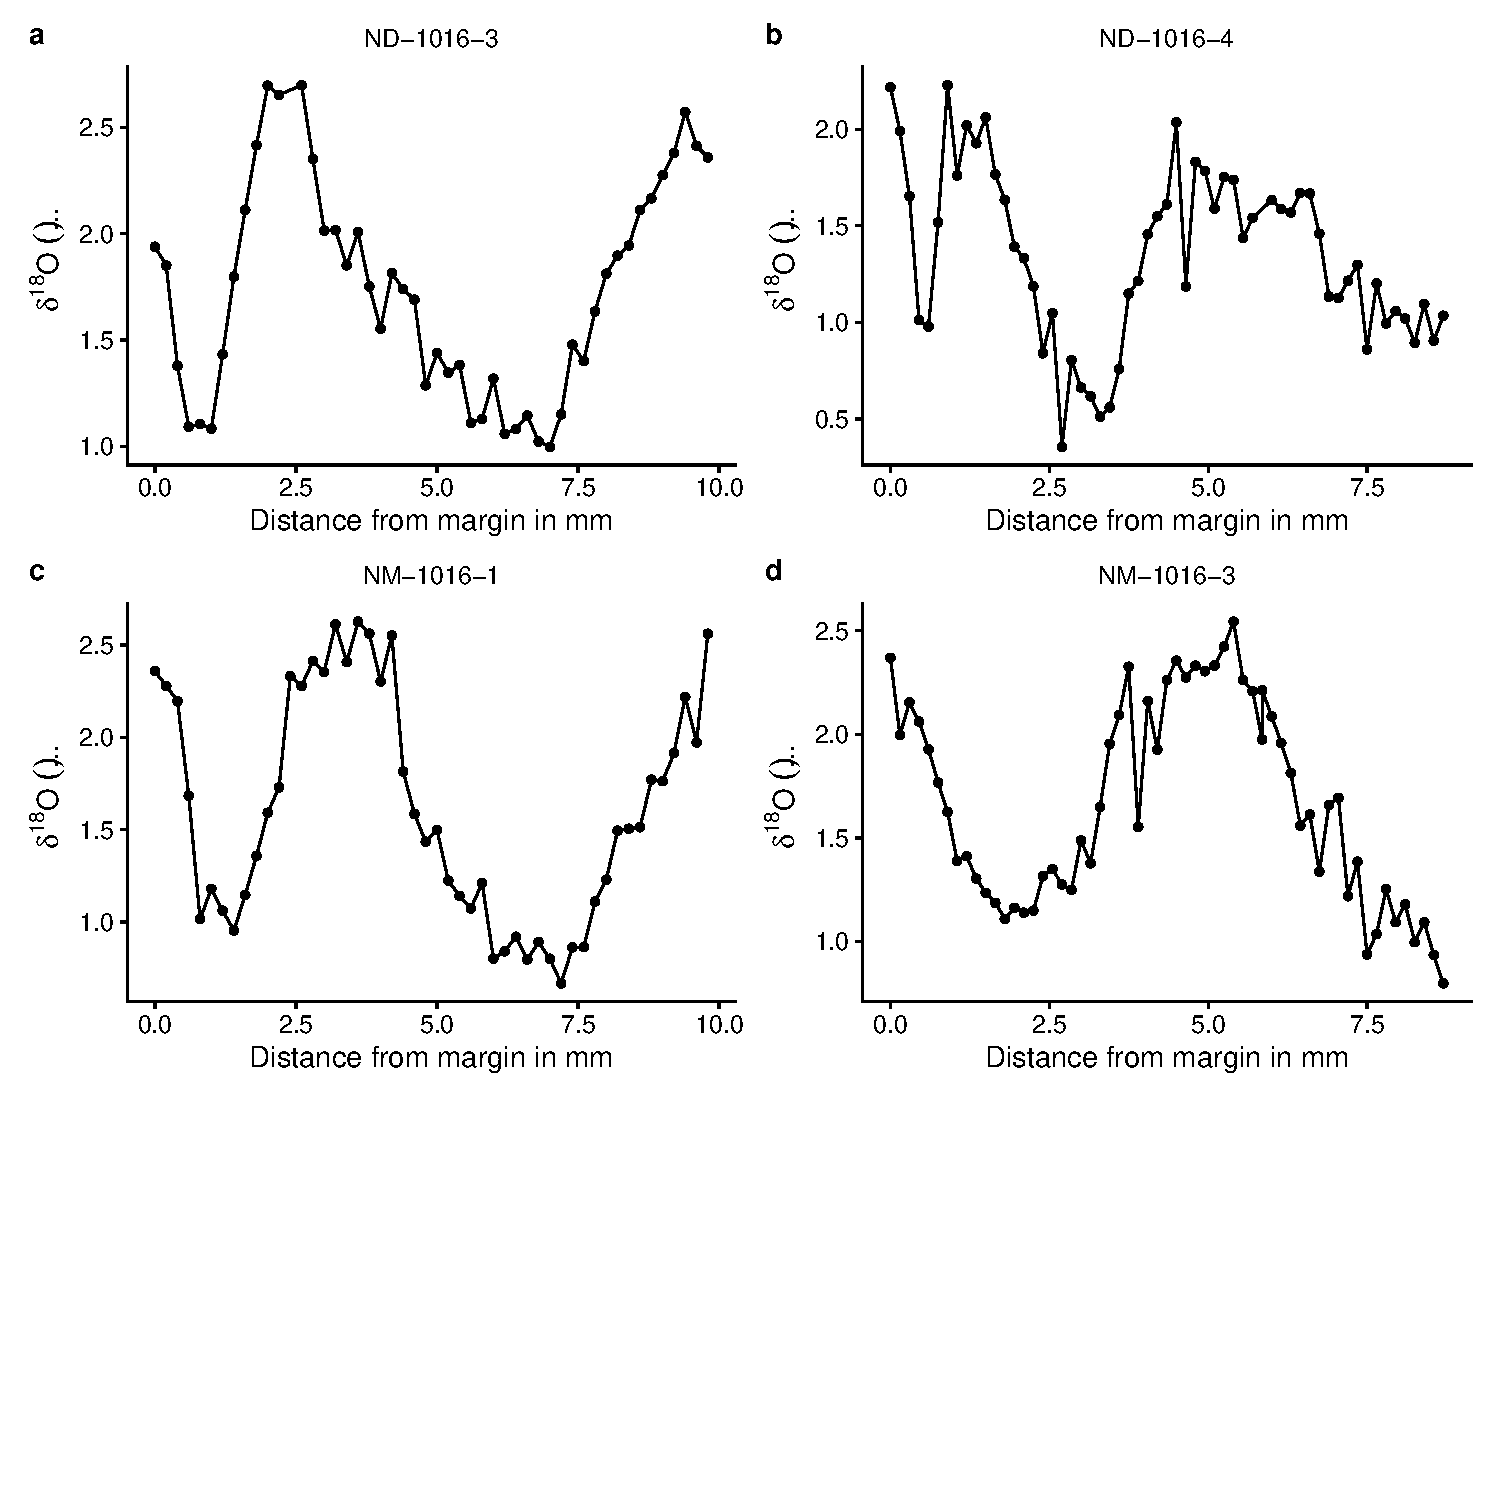
\includegraphics{Manuscript_files/figure-pdf/fig-Nac_iso-1.pdf}

}

\caption{\label{fig-Nac_iso}Isotope values of \emph{Nacella} sp. limpet
shells from Cambaceres Bay (\emph{a-f}).}

\end{figure}%

\begin{figure}

\centering{

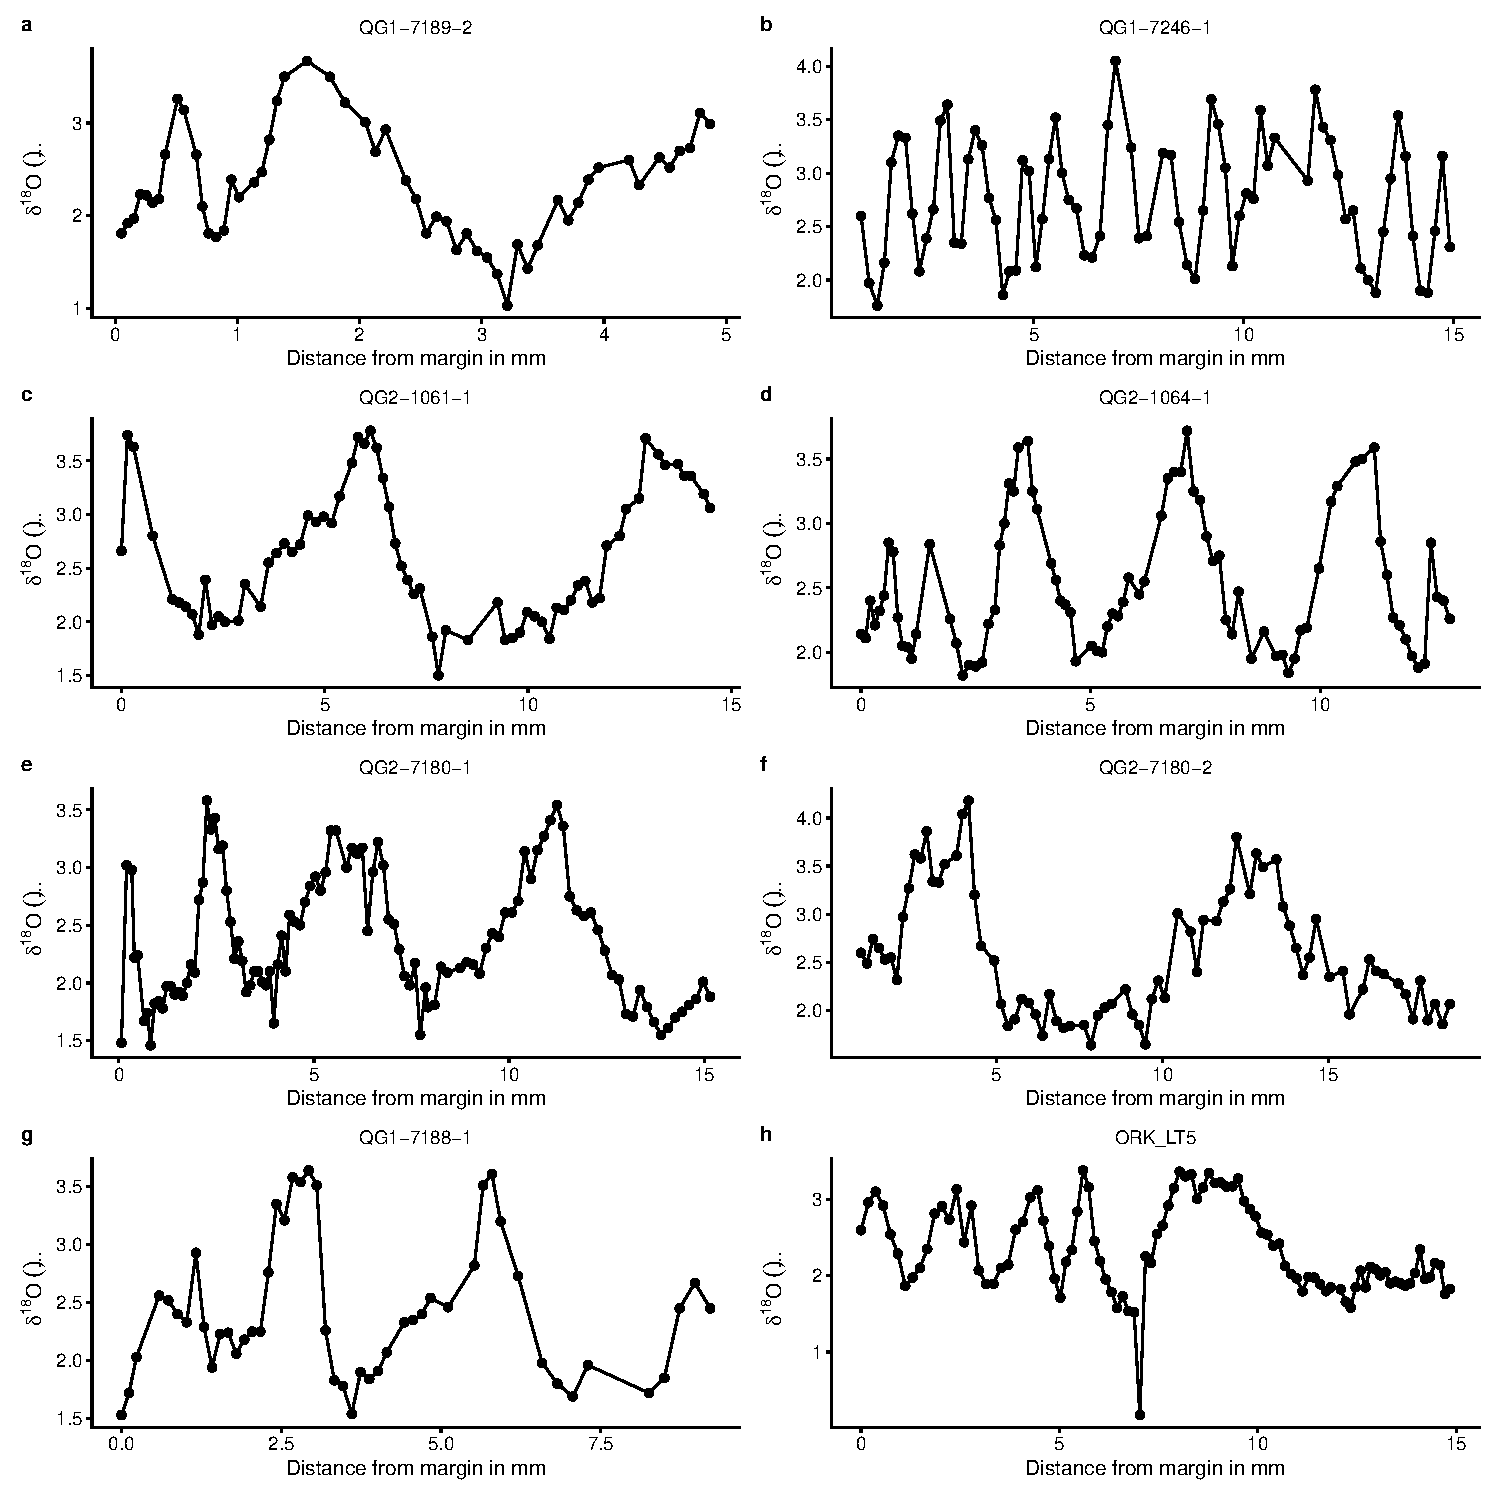
\includegraphics{Manuscript_files/figure-pdf/fig-Pat_iso-1.pdf}

}

\caption{\label{fig-Pat_iso}Isotope values of \emph{Patella vulgata}
limpet shells from Quoygrew (QG, \emph{a-g}) and Rack Wick Bay (ORK,
\emph{h}) on Westray, Orkney.}

\end{figure}%

\subsection{Dynamic Time Warping}\label{dynamic-time-warping}

Because the exact location used in the analysis of stable oxygen
isotopes is not possible to reconstruct for each carbonate powder
sample, we used dynamic time warping (DTW) to align the time series of
δ\textsuperscript{18}O-values and Mg/Ca ratios. DTW is an algorithm that
measures similarity between two proxy-sequences, which may vary in
sampling resolution or interval. By stretching or compressing sections
of the series, DTW finds the probable alignment between the two
sequences. This allows us to compare the proxy data sets more
effectively, ensuring that the temporal dynamics of each shell are
accurately matched despite possible discrepancies in sampling intervals
or rates. We applied the DTW algorithm using the \texttt{dtw} package in
R \citep{Giorgino2009-sj, R_Core_Team2020-mk}, which provides a robust
framework for aligning time series data. This involved selecting
appropriate distance measures and constraints to ensure meaningful
alignment. The process involved iterative adjustments to minimise the
overall distance between corresponding points in the two data sets. The
code used for this analysis as well as the data required to run it can
be found in this \textbf{OSF repository}.

\section{Results}\label{Results}

\subsection{\texorpdfstring{\emph{Patella
vulgata}}{Patella vulgata}}\label{patella-vulgata}

\begin{itemize}
\tightlist
\item
  Show one or a few of the LIBS maps as well as the line scans.
\item
  Show one the line scans together with isotope data.
\item
  Show correlation graphs.
\end{itemize}

\begin{figure}[H]

{\centering 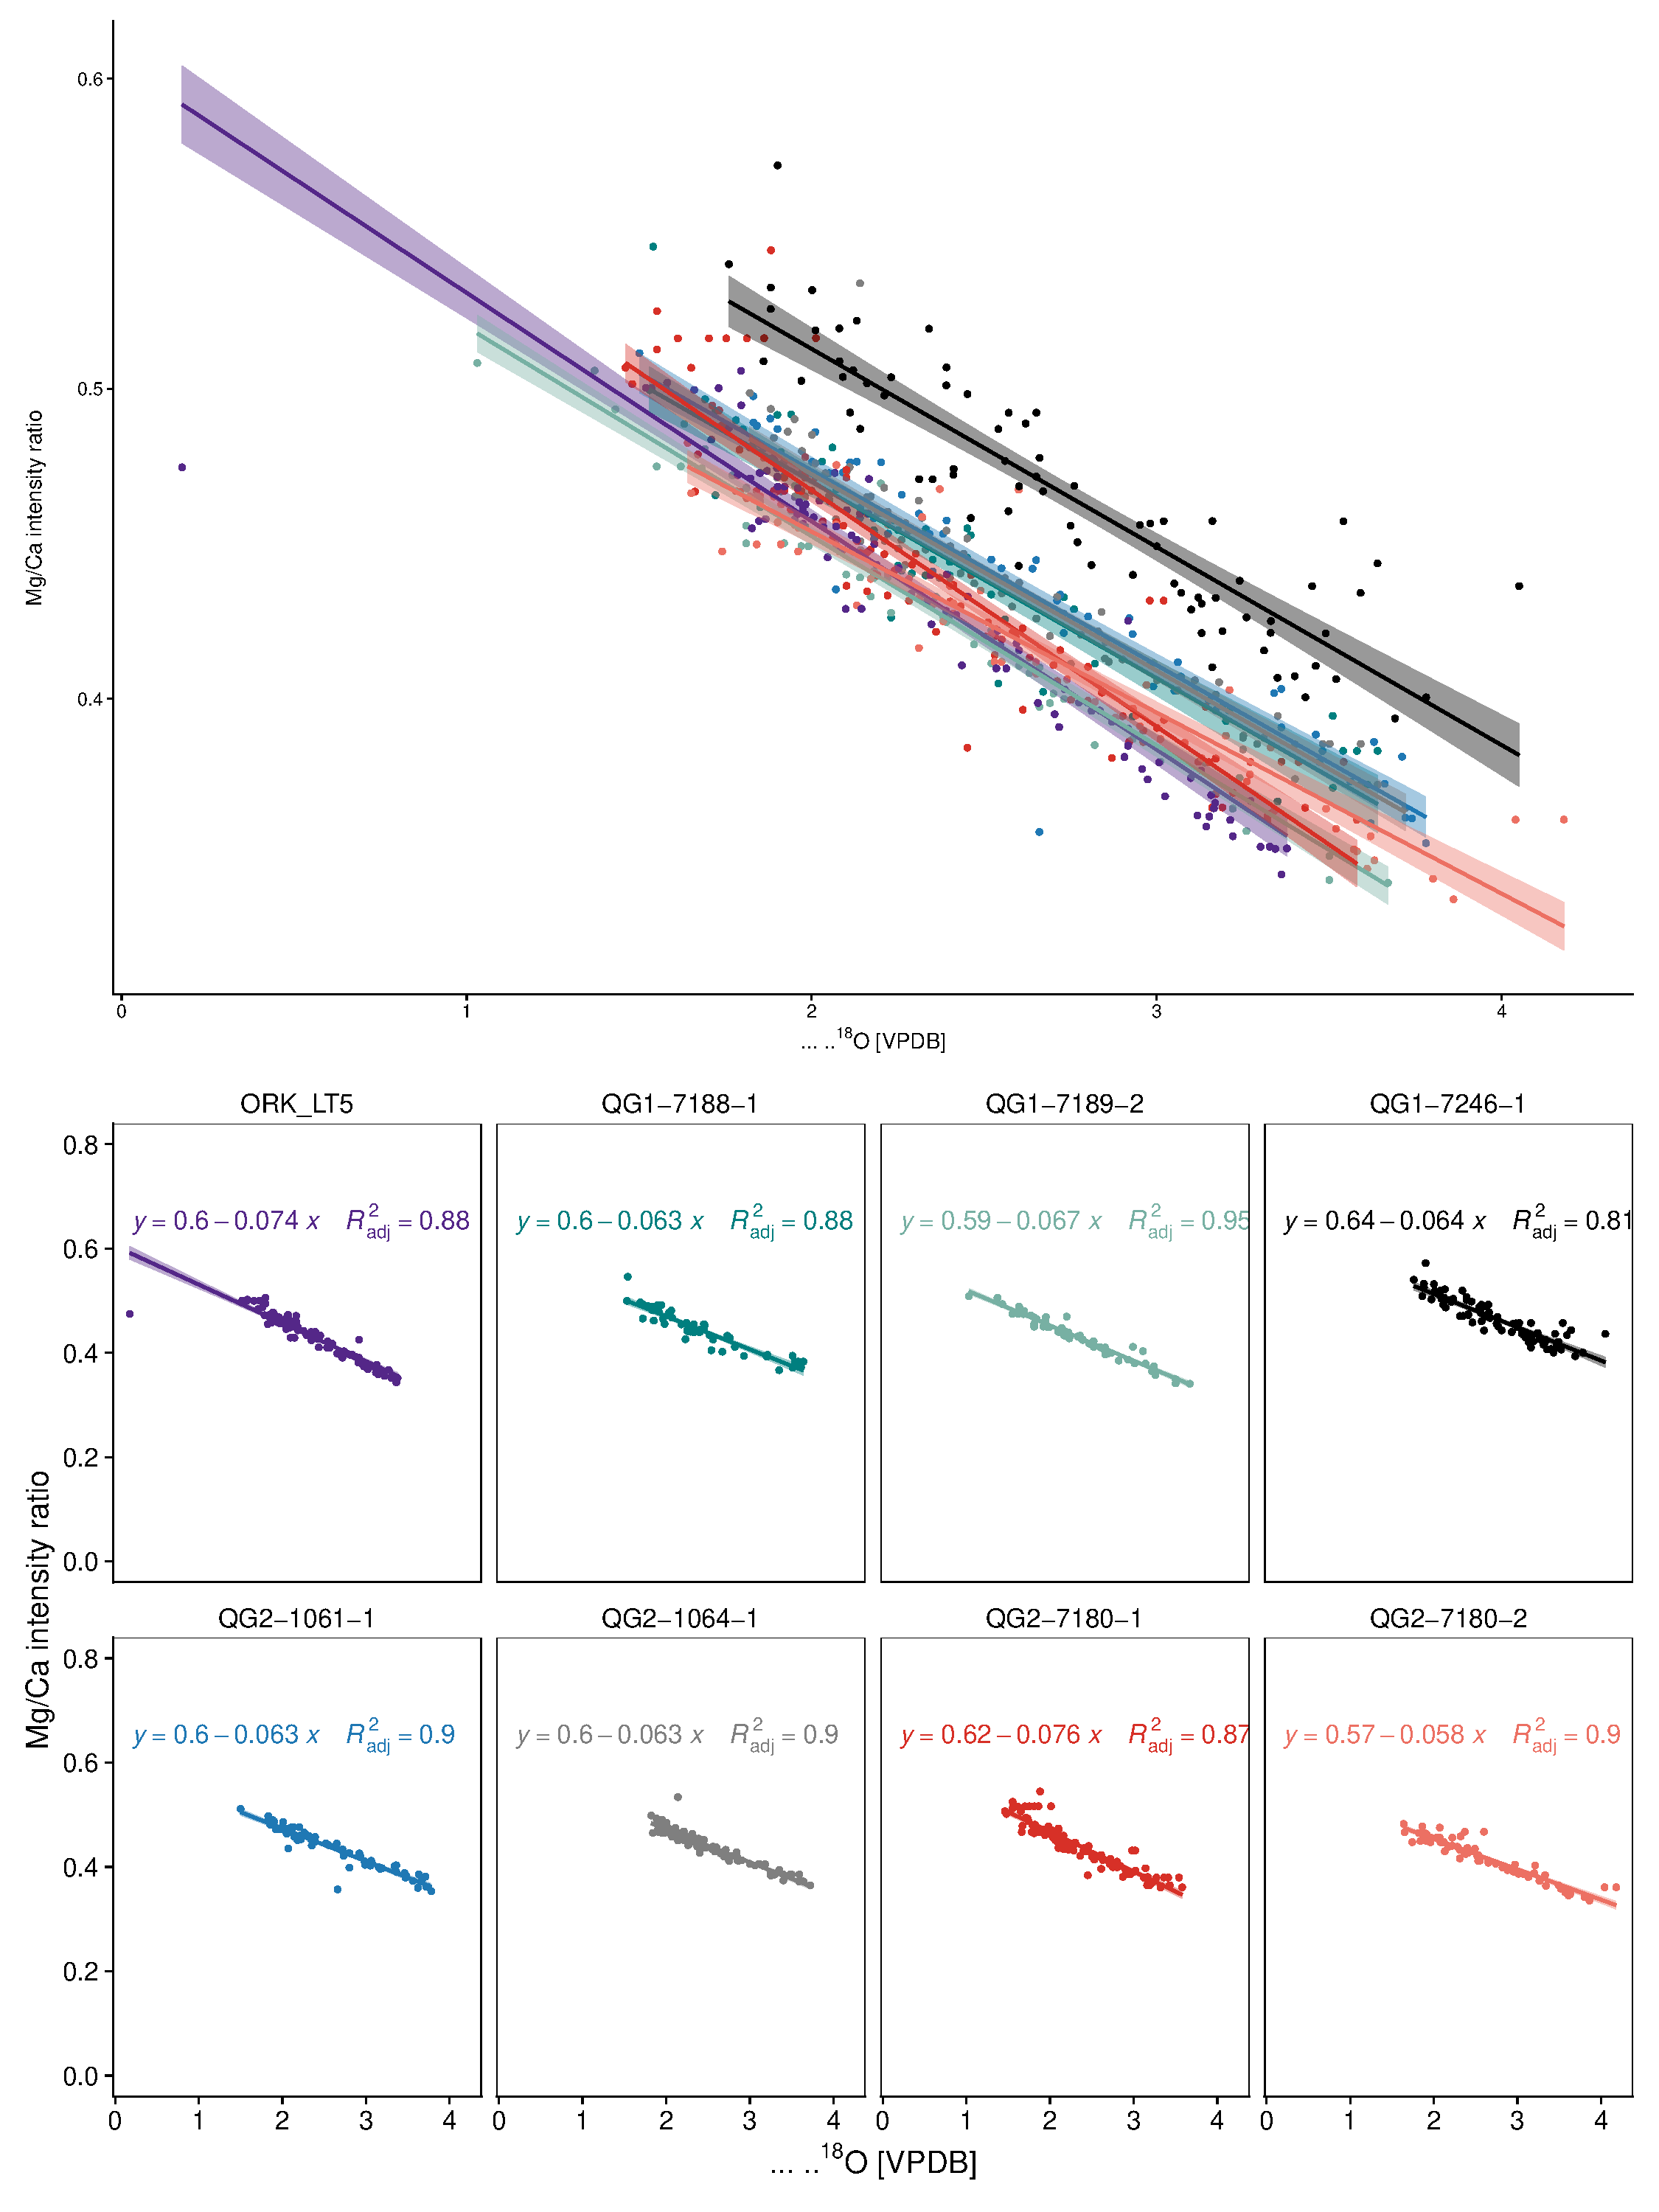
\includegraphics{Manuscript_files/figure-pdf/Patella_Correlation_Graphs-1.pdf}

}

\caption{Correlation graphs for \emph{Patella vulgata} specimens}

\end{figure}%

\subsection{\texorpdfstring{\emph{Nacella}
sp.}{Nacella sp.}}\label{nacella-sp.}

\begin{figure}[H]

{\centering 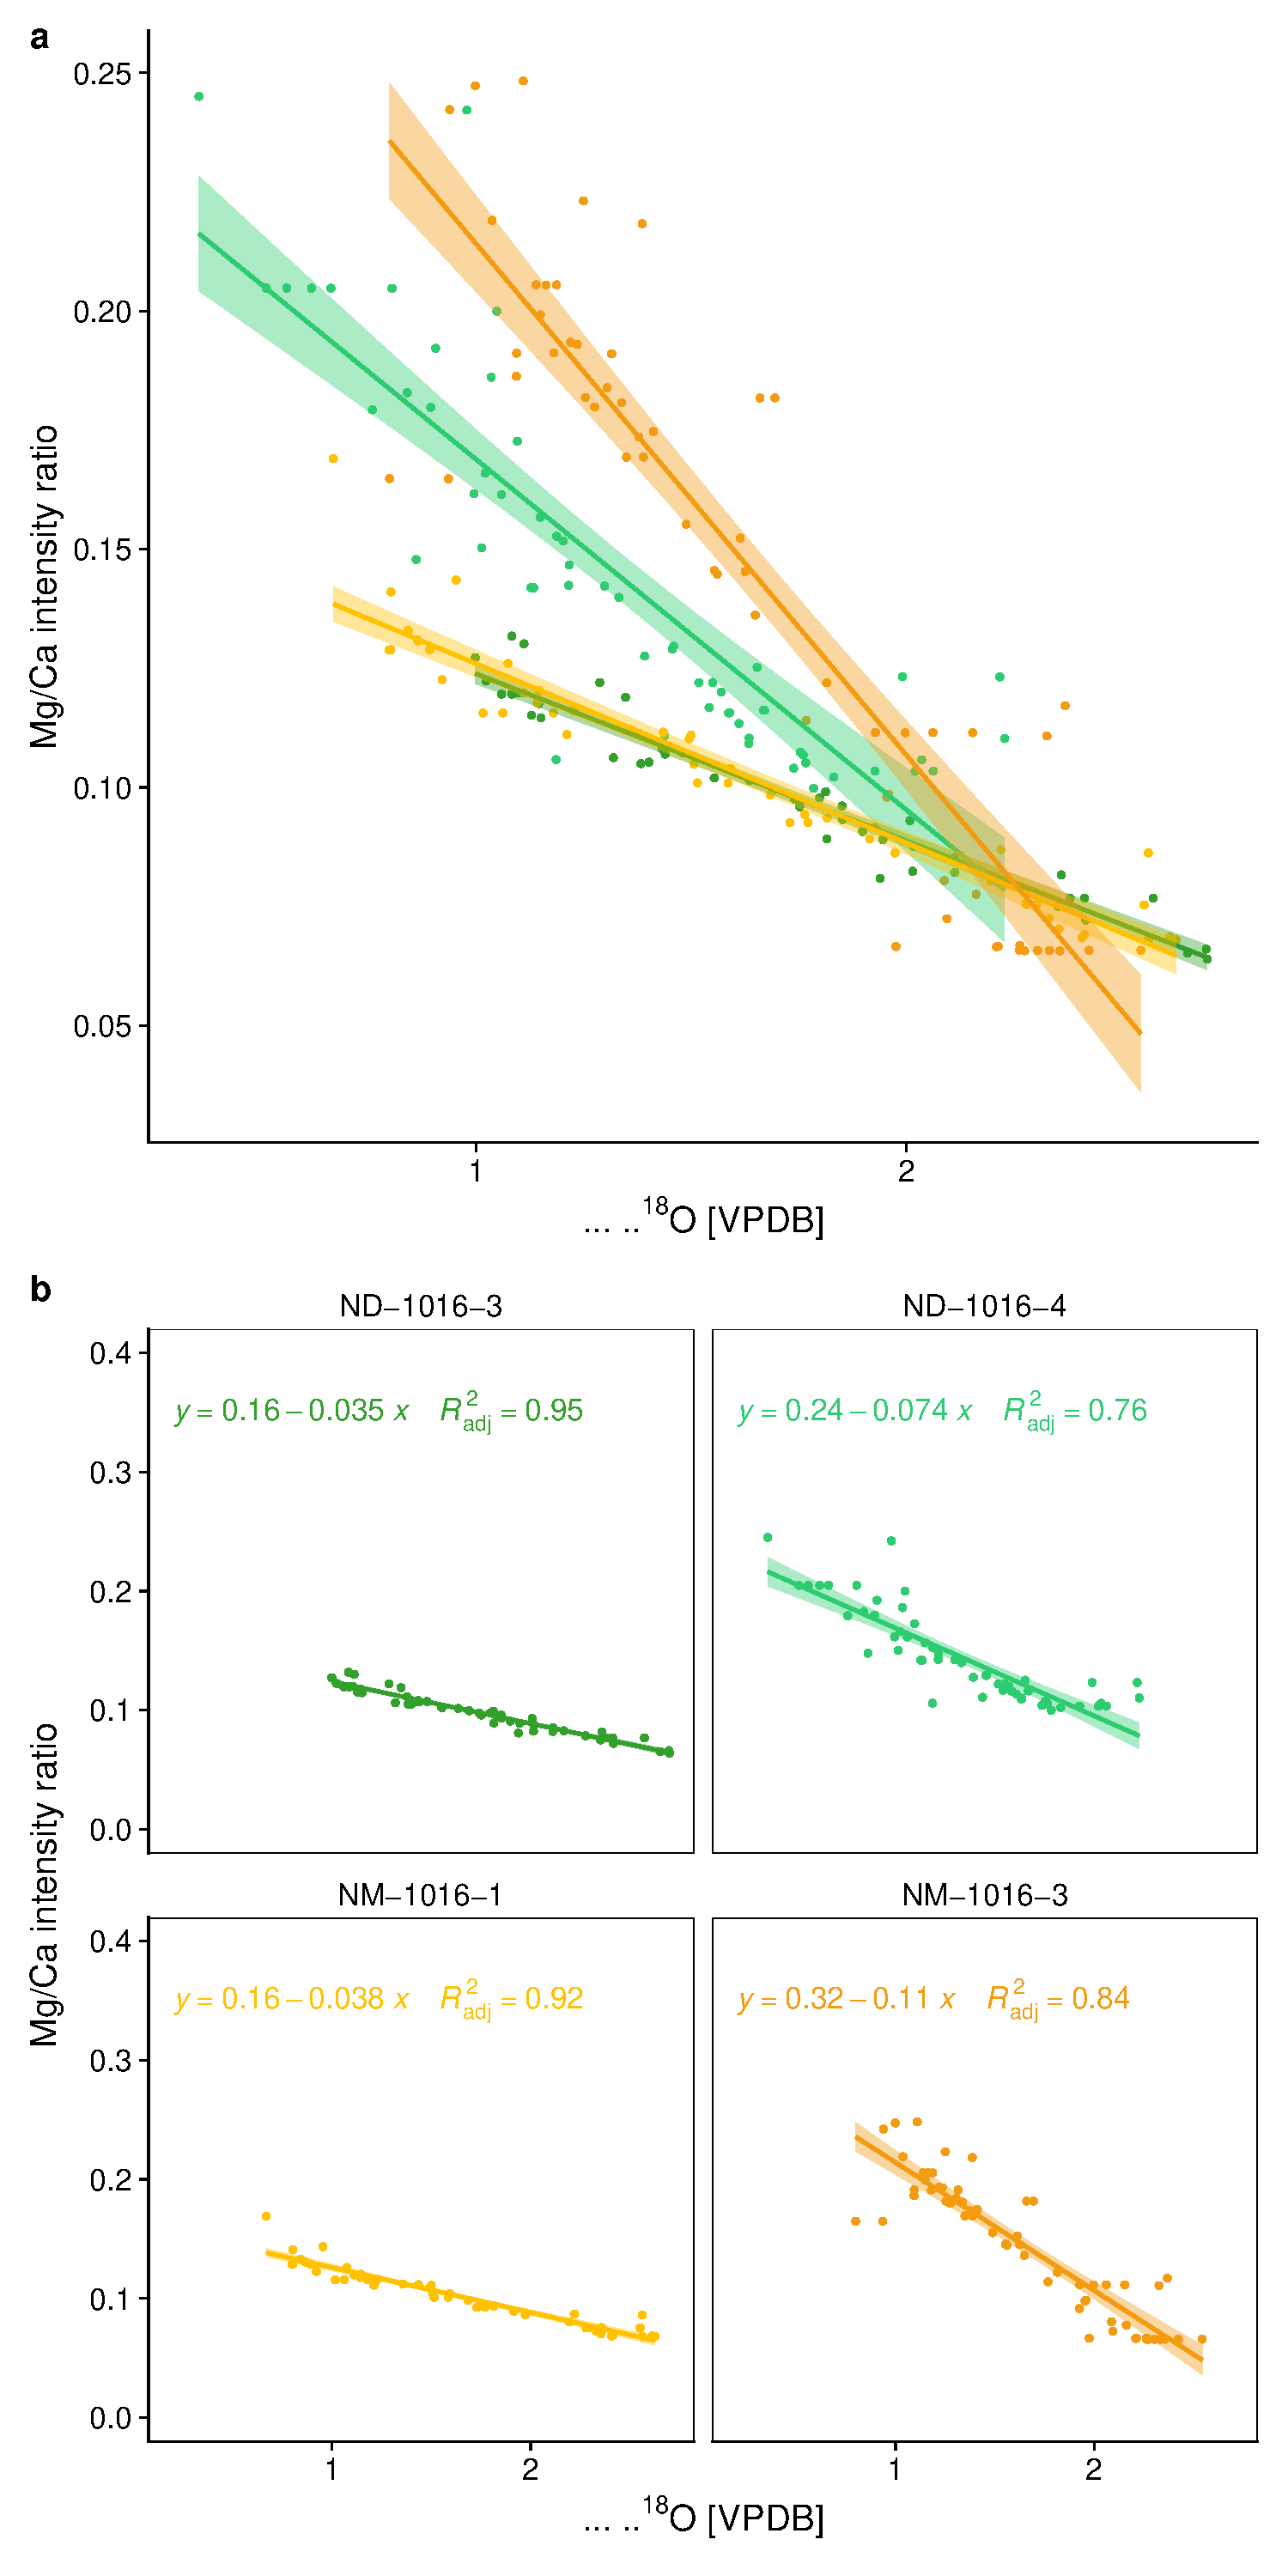
\includegraphics{Manuscript_files/figure-pdf/Nacella_Correlation_Graphs-1.pdf}

}

\caption{Correlation graphs for \emph{Nacella} sp. specimens}

\end{figure}%

\section{Discussion}\label{discussion}

\subsection{Other correlations}\label{other-correlations}

\begin{figure}[H]

{\centering 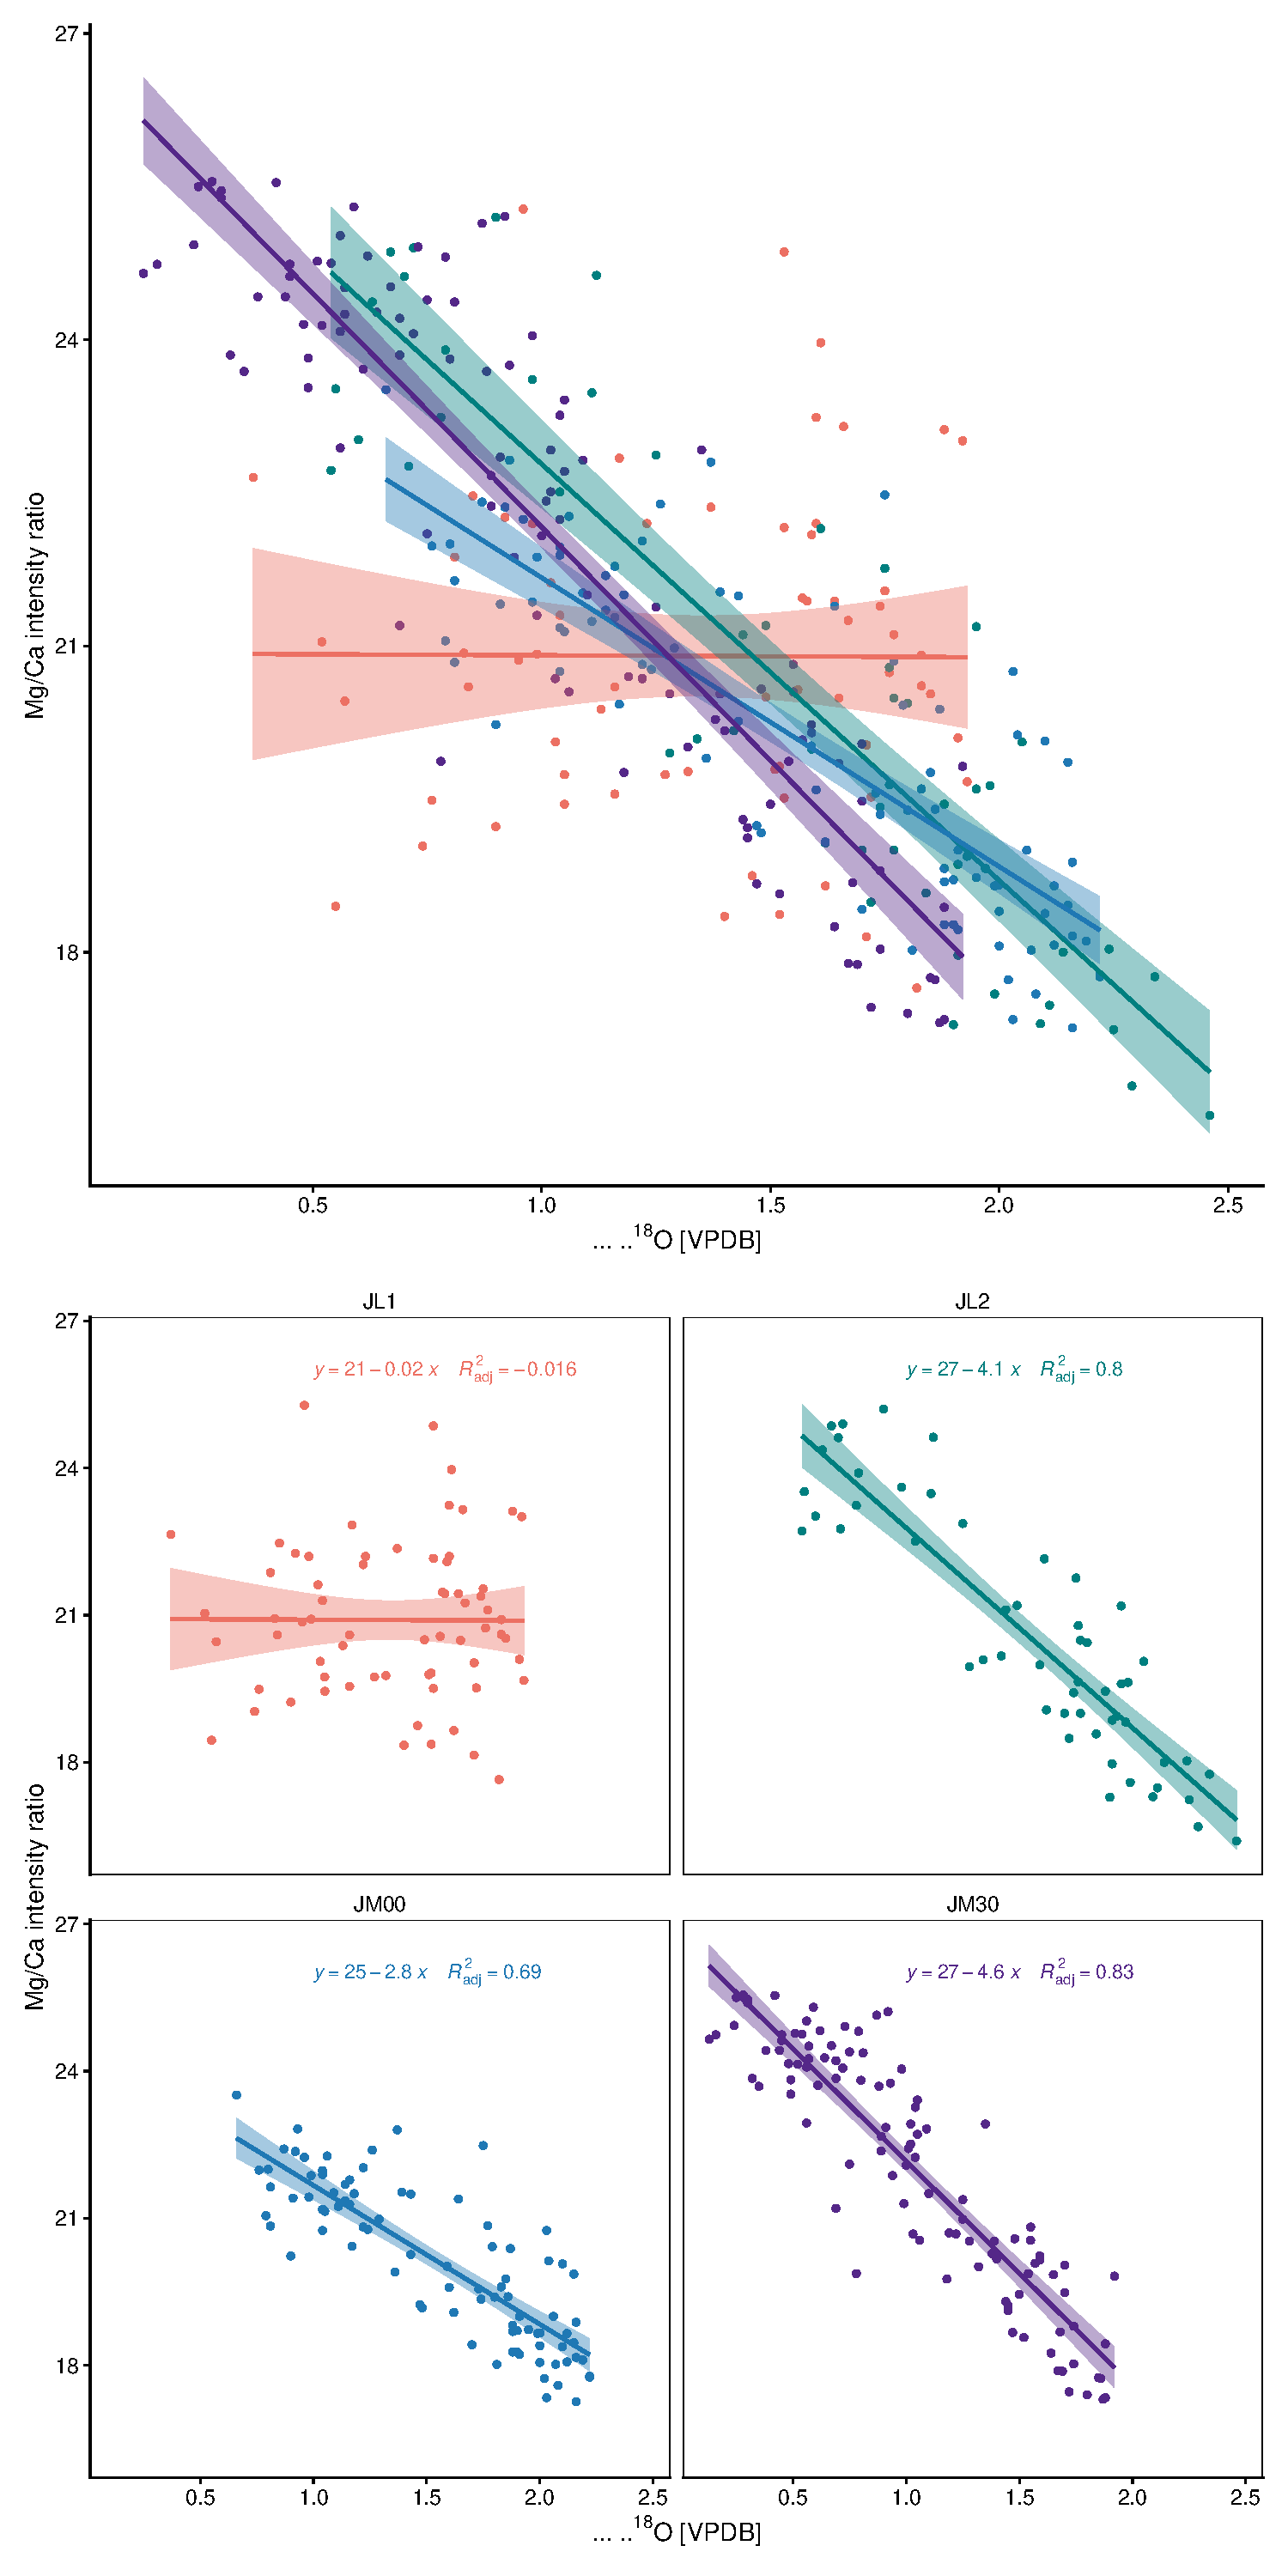
\includegraphics{Manuscript_files/figure-pdf/Ferguson Data-1.pdf}

}

\caption{Correlation graphs for Ferguson et al.~specimens}

\end{figure}%

\begin{longtable}[]{@{}
  >{\raggedright\arraybackslash}p{(\columnwidth - 8\tabcolsep) * \real{0.2000}}
  >{\raggedright\arraybackslash}p{(\columnwidth - 8\tabcolsep) * \real{0.2000}}
  >{\raggedright\arraybackslash}p{(\columnwidth - 8\tabcolsep) * \real{0.2000}}
  >{\raggedright\arraybackslash}p{(\columnwidth - 8\tabcolsep) * \real{0.2000}}
  >{\raggedright\arraybackslash}p{(\columnwidth - 8\tabcolsep) * \real{0.2000}}@{}}
\caption{Table 2: Overview of comparative correlations
\{\#tab:correlations\}}\tabularnewline
\toprule\noalign{}
\begin{minipage}[b]{\linewidth}\raggedright
Species
\end{minipage} & \begin{minipage}[b]{\linewidth}\raggedright
Locality
\end{minipage} & \begin{minipage}[b]{\linewidth}\raggedright
Specimen
\end{minipage} & \begin{minipage}[b]{\linewidth}\raggedright
Correlation R\textsuperscript{2}
\end{minipage} & \begin{minipage}[b]{\linewidth}\raggedright
Study
\end{minipage} \\
\midrule\noalign{}
\endfirsthead
\toprule\noalign{}
\begin{minipage}[b]{\linewidth}\raggedright
Species
\end{minipage} & \begin{minipage}[b]{\linewidth}\raggedright
Locality
\end{minipage} & \begin{minipage}[b]{\linewidth}\raggedright
Specimen
\end{minipage} & \begin{minipage}[b]{\linewidth}\raggedright
Correlation R\textsuperscript{2}
\end{minipage} & \begin{minipage}[b]{\linewidth}\raggedright
Study
\end{minipage} \\
\midrule\noalign{}
\endhead
\bottomrule\noalign{}
\endlastfoot
\emph{P. depressa} & Northern Spain & LAN541 & 0.87 &
\citep{Garcia-Escarzaga2021-ij} \\
& & LAN545 & 0.86 & \\
& & LAN554 & 0.78 & \\
& & LAN559 & 0.82 & \\
\emph{P. caerulea} & Croatia & ISTPC1 & 0.9 & \citep{Hausmann2019-fi} \\
& & ISTPC2 & 0.84 & \\
& Crete & AF1911A & 0.91\footnote{SST only, no other geochemical data
  available} & \\
& & AF3003A & 0.92\footnote{SST only, no geochemical data available}
& \\
& Israel & AKKPC2 & 0.96 & \\
& & AKKPC3 & 0.89 & \\
& & FRMPC1 & 0.84 & \\
& & FRMPC2 & 0.96 & \\
& Libya & MO31A & 0.83 & \\
& & MP64A & 0.33 & \\
& & MP67A & 0.96 & \\
& & MP68A & 0.81 & \\
& Malta & MA10 & 0.82 & \\
& Tunisia & TUNPC1 & 0.81 & \\
& & TUNPC2 & 0.78 & \\
& Turkey & ANTPC1 & 0.95 & \\
& & ANTPC2 & 0.93 & \\
& & KIZPC1 & 0.94 & \\
& & KIZPC2 & 0.86 & \\
\emph{P. rustica} & Gibraltar & JL1 & 0.02 & \citep{Ferguson2011-zl} \\
& & JL2 & 0.8 (0.79) & \\
\emph{P. caerulea} & Gibraltar & JM00 & 0.69 (0.79) & \\
& & JM30 & 0.83 (0.79) & \\
\emph{P. vulgata} & Orkney & ORK-LT5 & not reported, here 0.88 &
\citep{Graniero2017-io} and this study \\
& & & & \\
& & & & \\
& & & & \\
\end{longtable}

\subsection{Comparison of ORK-LT5}\label{comparison-of-ork-lt5}

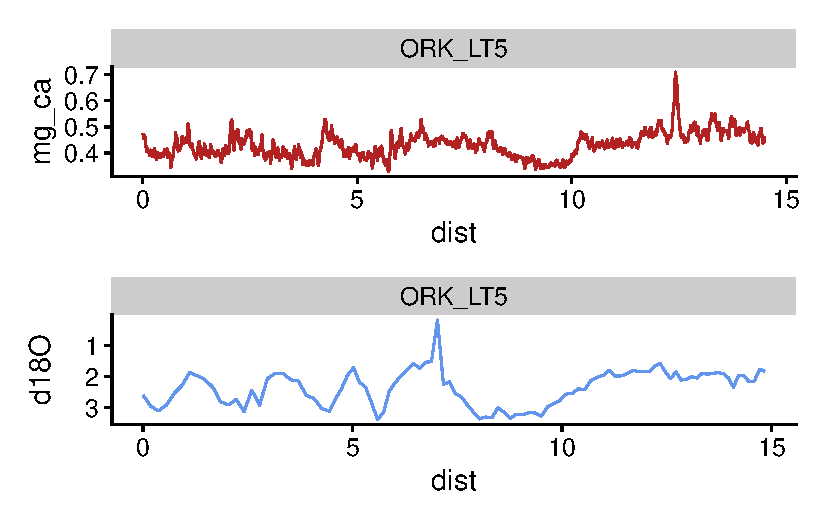
\includegraphics{Manuscript_files/figure-pdf/unnamed-chunk-1-1.pdf}

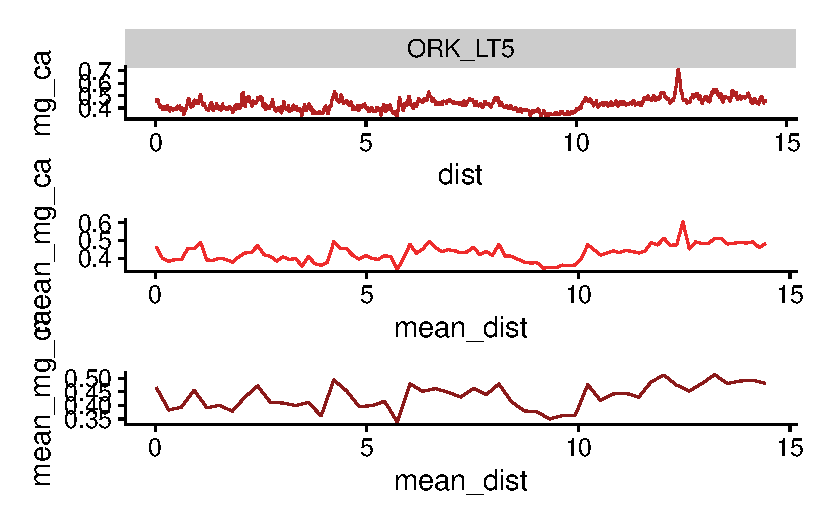
\includegraphics{Manuscript_files/figure-pdf/subsample-1.pdf}


\renewcommand\refname{References}
  \bibliography{bibliography.bib}


\end{document}
